\documentclass[11pt,a4paper]{article}


% font
%\usepackage{fontspec}
%\setmainfont{Times New Roman}
%\usepackage{tgschola}

\usepackage{helvet}
\renewcommand{\familydefault}{\sfdefault}

\usepackage[margin=0.8in]{geometry}
\usepackage[utf8]{inputenc}
\usepackage{amsmath}
\usepackage{amsfonts}
\usepackage{amssymb}

% https://www.sharelatex.com/learn/Hyperlinks
\usepackage{hyperref}
\hypersetup{
    colorlinks=true,
    linkcolor=blue9,
    filecolor=magenta,      
    urlcolor=red,
}
 
\usepackage{float}

\usepackage{lipsum}% http://ctan.org/pkg/lipsum

%% Bibliography/references packages
\usepackage[comma]{natbib}
%%\bibliographystyle{agsm}
\bibliographystyle{dcu}

%% https://en.wikibooks.org/wiki/LaTeX/List_Structures
\usepackage{scrextend}

% tables, row colour
\usepackage{tabularx,colortbl}
% For vertical centering text in X column
\renewcommand\tabularxcolumn[1]{m{#1}}

% https://tex.stackexchange.com/questions/22751/how-to-force-table-caption-on-top
%\usepackage[tableposition=top]{caption}
\usepackage{float}
\floatstyle{plaintop}
\restylefloat{table}

% https://en.wikibooks.org/wiki/LaTeX/List_Structures
\usepackage{enumitem}

% https://jansoehlke.com/2010/06/strikethrough-in-latex/
\usepackage{ulem}

% Code highlighting
\usepackage[outputdir=build]{minted}

%% Report variables
\newcommand{\scname}{PRCO304}
\newcommand{\dlatestv}{7.00}


\definecolor{babyblueeyes}{rgb}{0.63, 0.79, 0.95}
\definecolor{ballblue}{rgb}{0.13, 0.67, 0.8}
\definecolor{beaublue}{rgb}{0.74, 0.83, 0.9}
\definecolor{blue8}{rgb}{0.09, 0.39, 0.67}
\definecolor{blue9}{rgb}{0.00, 0.30, 0.51}
\definecolor{blue9d}{rgb}{0.00, 0.21, 0.36}


%\usepackage{etoolbox}
%\patchcmd{\chapter}{\thispagestyle{plain}}{\thispagestyle{fancy}}{}{}

%https://tex.stackexchange.com/questions/75667/change-colour-on-chapter-section-headings-lyx
\usepackage{sectsty}
\chapterfont{\color{blue9d}}
\sectionfont{\color{blue9d}}
\subsectionfont{\color{blue9d}}
%\allchapterfont{\itshape}

\usepackage{titlesec}

\usepackage{array,booktabs,arydshln,xcolor}
\usepackage{xcolor}% http://ctan.org/pkg/xcolor
\usepackage{fancyhdr}% http://ctan.org/pkg/fancyhdr
\fancypagestyle{plain}{%
	\renewcommand{\headrulewidth}{3pt}
	\renewcommand{\headrule}{\hbox to\headwidth{%
		\color{blue9}\leaders\hrule height \headrulewidth\hfill}}
	\renewcommand{\footrulewidth}{3pt}
	\renewcommand{\footrule}{\hbox to\headwidth{%
		\color{blue9}\leaders\hrule height \headrulewidth\hfill}}
	
	%\fancyhf{}
	%\fancyhead[LE]{\textbf{\leftmark}}
	%\fancyhead[RE]{\textbf{\scname{}}}
	%\fancyhead[LO]{\textbf{\scname{}}}
	%\fancyhead[RO]{\textbf{\rightmark}}

	%\fancyfoot[LE]{\textbf{\thepage}}
	%\fancyfoot[RE]{\textbf{\scname{} Configuration Guide}}
	%\fancyfoot[LO]{\textbf{\scname{} Configuration Guide}}
	%\fancyfoot[RO]{\textbf{\thepage}}
}


%% Make bibliography show in table of contents
%% https://tex.stackexchange.com/questions/8458/making-the-bibliography-appear-in-the-table-of-contents
\usepackage[nottoc,numbib]{tocbibind}
%% ^^^ overwrites \bibname, so set it back
\renewcommand{\bibname}{References}

\RequirePackage{filecontents}
\begin{filecontents}{prco304_h4.bib}
@online{wikipedia:dft,
  author = {Wikipedia},
  title = {Discrete Fourier transform},
  year = 2018,
  url = {https://en.wikipedia.org/wiki/Discrete\_Fourier\_transform},
  urldate = {2018-01-15}
}
@online{server:gpu,
  author = {Amazon AWS},
  title = {Introducing Amazon EC2 P2 Instances, the largest GPU-Powered virtual machine in the cloud},
  year = 2018,
  url = {https://aws.amazon.com/about-aws/whats-new/2016/09/introducing-amazon-ec2-p2-instances-the-largest-gpu-powered-virtual-machine-in-the-cloud/},
  urldate = {2016-09-26}
}
@misc{scarabhardware,
title={MiniSpartan6+}, 
journal={{Scarab Hardware}},
url={https://www.scarabhardware.com/minispartan6/},
year=2014
}
@misc{arty,
title={Arty Artix-7 FPGA Development Board}, 
journal={{Avnet}},
url={https://uk.rs-online.com/web/p/programmable-logic-development-kits/1346478/},
year=2015
}
@misc{arndt2002algorithms,
  title={Algorithms For Programmers},
  author={Arndt, J{\"o}rg},
  year = 2002
}
@book{hdl,
title={HDL Programming Fundamentals: VHDL and Verilog},
author={Nazeih Botros},
year={2006},
publisher={Da Vinci Engineering Press}
}

@misc{arm, title={ARM in the World of FPGA-Based Prototyping}, url={https://community.arm.com/processors/b/blog/posts/arm-in-the-world-of-fpga-based-prototyping}, journal={Arm Community},
year={2016}}

@book{microblaze,
title={MicroBlaze 
Processor Reference 
Guide},
journal={Xilinx},
year={2017}
} 

\end{filecontents}

%s comments
\usepackage{verbatim}

%inline graphs
\usepackage{wrapfig}
% multiple figures on line
\usepackage{subfig}

\usepackage{graphicx}
\graphicspath{ {img/} }

% Caption font size
% https://tex.stackexchange.com/questions/86120/font-size-of-figure-caption-header
\usepackage[font=scriptsize,labelfont=bf]{caption}

%\setlength{\belowcaptionskip}{-10pt}
%\setlength{\abovecaptionskip}{-5pt} % Chosen fairly arbitrarily


\usepackage{fancyhdr}
\pagestyle{fancy}
\lhead{\rightmark}
\chead{}
\rhead{Highlight Report Document (Rev. \dlatestv{})}
\lfoot{Page \thepage}
\cfoot{}
\rfoot{Ben Lancaster 10424877}

\renewcommand{\subsectionmark}[1]{\markright{\thesubsection\ #1}}


\begin{document}

\begin{titlepage}
\begin{center}

\vspace*{5cm}
\Large
\textbf{
%%PRCO304 - Project Initiation Document
%Highlight Reports
{\color{blue9d}Highlight Report Document (Rev. \dlatestv{})}
}

\vspace{0.4cm}
\large
%%Space optimised FPGA-based side-microprocessor.
PRCO304 - FPGA-based RISC microprocessor
%%EMBEDDED CPU - FPGA-based RISC microprocessor

\vspace{4cm}
\textbf{Ben Lancaster}\\
\today 


\end{center}

\end{titlepage}

\pagestyle{plain}

\section*{Revision History}
\begin{table}[h]
\def\arraystretch{1.5}%  1 is the default, change whatever you need
    \begin{tabularx}{\textwidth}{|l|l|X|}
    \hline
    Date & Highlight & Changes \\
	\specialrule{2pt}{-2pt}{0pt}
	21/03/2018 & 7 & Highlight report 7. \\ \hline
	15/03/2018 & 6 & Highlight report 6. \\ \hline
	07/03/2018 & 5 & Highlight report 5.\newline Added Highlight Attachments section. 
	\\ \hline
	28/02/2018 & 4 & Highlight report 4. \\ \hline
	20/02/2018 & 3 & Highlight report 3.\newline Added Risks \& Challenges section.\newline Changed header (right) title. \\ \hline
	14/02/2018 & 2 & Highlight report 2. \\ \hline
	06/02/2018 & 1 & Highlight report 1. \\ \hline
    \end{tabularx}
    \caption{Document revisions.}
\end{table}
\newpage

\renewcommand*\contentsname{Table of Contents}

{\hypersetup{linkcolor=black}
\tableofcontents
}
\newpage

\section{Highlight Reports}
\subsection{Highlight Report 1}
\begin{table}[H]
\def\arraystretch{1.5}%  1 is the default, change whatever you need
    \begin{tabularx}{\textwidth}{|X|}
    \hline 
	\multicolumn{1}{|c|}{\textbf{PRCO304: Highlight Report 1}}
    \\
	\specialrule{2pt}{-2pt}{0pt}
    \textbf{Name:} Ben Lancaster
    \\ \specialrule{2pt}{-2pt}{0pt}
	\textbf{Date:} 06/02/2018
	\\ \specialrule{2pt}{-2pt}{0pt}
	\textbf{Active project stage:} Stage 1.1:  Research  and  Requirement Gathering
	\\ \specialrule{2pt}{-2pt}{0pt}
	\textbf{Review of work undertaken:}\newline
	This week was assigned to work on stage 1.1:  Research  and  requirement
gathering. \newline\newline
	\textbf{Research and requirement gathering:}\newline
	Research into existing soft-core processor designs has been started to identify their features, targets, and advantages and disadvantages. Key existing soft-core processors found are:\newline
	-  Xilinx' MicroBlaze: a 32-bit Xilinx FPGA embeddable core capable of running operating systems, like Linux. Exposes a configurable GUI to customise the build of the processor to suit designers requirements (like number of GPIO, interrupts, timers, etc.).\newline
	- ARM Cortex-A9: a 32-bit Xilinx and Altera FPGA core. Features out-of-order execution, compatible with existing ARM Thumb2 C compilers, and multi-core processing.\newline\newline
	I have used this research to aim my soft-core processor's requirements and architecture. To document and finalize my processors design and requirements, I have started a processor specification and reference document. This document outlines the processors features, architecture, compatibility, and instructions.
	\newline\newline
	Additional progress:\newline
	- Version control set up for documentation, highlight reports, and code bases.
		
	\\ \hline
	\textbf{Risks and Challenges:}\newline
	{\color{red} Urgent risks:}\newline
	{\color{orange} New risks:}\newline
	{\color{purple} Existing risks:\newline
	RC4: Schedule overrun. A gantt time chart has been created to better visualize task durations and requirements.}\newline
	\\ \hline
	\textbf{Plan of work for the next week:}\newline
	Work will begin on Stage 1.2: Core high level design.\newline\newline
	Finalised specifications and architecture of the soft-core processor will be put into a processor specification and reference document.
	\newline
	Architecture, control, pipelines, will be visualised in this document.
	
	\\ \hline
	\textbf{Date(s) of supervisory meeting(s) since last Highlight:}\newline
	This is the 1st highlight report.\newline
	30/01/18 - An introductory meeting was held to discuss the project initiation document (PID) and gain feedback on the project.
	\\ \hline
	\textbf{Notes from supervisory meeting(s) held since last Highlight:}\newline
	Ensure risks are carefully explored and project core deliverables are realistic and achievable.
	\\ \hline
    \end{tabularx}
    %\caption{Document revisions.}
\end{table}


\subsection{Highlight Report 2}
\begin{table}[H]
\def\arraystretch{1.5}%  1 is the default, change whatever you need
    \begin{tabularx}{\textwidth}{|X|}
    \hline 
	\multicolumn{1}{|c|}{\textbf{PRCO304: Highlight Report 2}}
    \\
	\specialrule{2pt}{-2pt}{0pt}
    \textbf{Name:} Ben Lancaster
    \\ \specialrule{2pt}{-2pt}{0pt}
	\textbf{Date:} 15/02/2018
	\\ \specialrule{2pt}{-2pt}{0pt}
	\textbf{Active project stage:} Stage 1.2:  Core high level design
	\\ \specialrule{2pt}{-2pt}{0pt}
	\textbf{Review of work undertaken:}\newline
	This week was assigned to work on stage 1.2:  Core high level design.
gathering. \newline\newline
	\textbf{Core high level design:}\newline
	I have spent this week defining a processor specification and creating a processor specification/reference guide booklet (see attached). This booklet will contain both high-level and technical details regarding the design and implementation of the processor, including: register sets, control and pipelining strategies, the ISA and each instruction, and the compiler and how to use it.	
	\newline\newline
	This booklet will be developed over the life cycle of the project. Although the specification has been clearly defined, the booklet will be incrementally updated as processor features/requirements are added to the implementation (such as instructions, modules, and compiler features).
	\newline\newline
	Currently the reference booklet contains: register set definitions, several primitive instructions, and a brief introduction to instruction cycle timing.
	
	\\ \hline
	\textbf{Risks and Challenges:}\newline
	{\color{red} Urgent risks:}\newline
	{\color{orange} New risks:}\newline
	{\color{purple} Existing risks:\newline
	\sout{RC4: Schedule overrun. A gantt time chart has been created to better visualize task durations and requirements.}}\newline
	{\color{gray} Resolved risks:\newline
	RC4: Schedule overrun. A gantt time chart has been created to better visualize task durations and requirements. (See attached time management chart indev.)}\newline
	\\ \hline
	\textbf{Plan of work for the next week:}\newline
	Work will begin on Stage 2.0: Core dev. Register set implementation.\newline\newline
	The register set module will be implemented in Verilog for the processor. Unit tests will be created to verify the timing/behaviour of the module.
	\newline
	The processor specification/reference booklet will be updated to describe how the register set has been implemented in the processor.
	
	\\ \hline
	\textbf{Date(s) of supervisory meeting(s) since last Highlight:}\newline
	08/02/18 15:00 - 15:40
	\\ \hline
	\textbf{Notes from supervisory meeting(s) held since last Highlight:}\newline
	Discussion included comparing existing processor's (ARM, x86) features (privileged instructions, interrupts, IO, variable-length ISA) and designs (ISA and pipelining) to this processor.
	\\ \hline
    \end{tabularx}
    %\caption{Document revisions.}
\end{table}

\subsection{Highlight Report 3}
\begin{table}[H]
\def\arraystretch{1.5}%  1 is the default, change whatever you need
    \begin{tabularx}{\textwidth}{|X|}
    \hline 
	\multicolumn{1}{|c|}{\textbf{PRCO304: Highlight Report 3}}
    \\
	\specialrule{2pt}{-2pt}{0pt}
    \textbf{Name:} Ben Lancaster
    \\ \specialrule{2pt}{-2pt}{0pt}
	\textbf{Date:} 20/02/2018
	\\ \specialrule{2pt}{-2pt}{0pt}
	\textbf{Active project stage:} Stage 2.0:  Core Register-set Implementation.
	\\ \specialrule{2pt}{-2pt}{0pt}
	\textbf{Review of work undertaken:}\newline
	This week was assigned to work on stage 2.0:  Core Register-set Implementation.
	\newline\newline
	\textbf{Core Register-set Implementation:}\newline
	Good progress has been made implementing the PRCO processor's register set in Verilog. The register set consists of 8 16-bit wide general purpose registers labelled rA through rH in duel-port read and single-port write.
	\newline\newline
	Implementation progress is approximately 1 week ahead of schedule. Because of this, work has also been done on the decoder and ALU modules.
	\newline\newline
	Consideration of the control/sequencing pipeline has been considered. The pipeline needs to work for time-varying functions (such as memory writes). The current plan is to give each module outputs to signal when it has finished so the following module can safely read in data and operate on it. A handshake between modules currently seems overkill due to the relatively simple structure but may be considered later in the project.
	
	\\ \hline
	\textbf{Risks and Challenges:}\newline
	{\color{red} Urgent risks:}\newline
	{\color{orange} New risks:\newline
	RC5: Complex memory operations (PUSH, POP) may require multiple instructions. PUSH/POP might be split into: (1) Inc/dec stack pointer; (2) Read RAM[stack pointer]. The compiler will be able to resolve this issue.}\newline
	{\color{purple} Existing risks:}\newline
	{\color{gray} Resolved risks:}\newline
	\\ \hline
	\textbf{Plan of work for the next week:}\newline
	Work will begin on Stage 2.1: Core dev. Decoder implementation.\newline\newline
	Some progress has already made but the decoder is not finished.
	\newline
	The processor specification/reference booklet will continued to be updated with implementation specific details of the processor.
	\\ \hline
	\textbf{Date(s) of supervisory meeting(s) since last Highlight:}\newline
	13/02/18 09:40
	\\ \hline
	\textbf{Notes from supervisory meeting(s) held since last Highlight:}\newline
	This discussions was over email; it was decided that a physical meeting would not be beneficial as the current project stage was starting the \textit{PRCO Processor Reference Guide} booklet. Progress on the booklet was shared and a brief overview of the {\color{ballblue}Register-set} and {\color{ballblue}Decoder} implementation.
	\\ \hline
    \end{tabularx}
    %\caption{Document revisions.}
\end{table}

\newpage
\subsection{Highlight Report 4}
\begin{table}[H]
\def\arraystretch{1.5}%  1 is the default, change whatever you need
    \begin{tabularx}{\textwidth}{|X|}
    \hline 
	\multicolumn{1}{|c|}{\textbf{PRCO304: Highlight Report 4}}
    \\
	\specialrule{2pt}{-2pt}{0pt}
    \textbf{Name:} Ben Lancaster
    \\ \specialrule{2pt}{-2pt}{0pt}
	\textbf{Date:} 28/02/2018
	\\ \specialrule{2pt}{-2pt}{0pt}
	\textbf{Active project stage:}\newline
	Stage 2.1:  Core: Register-set Implementation.\newline
	Stage 2.2:  Core: ALU, RAM Implementation.\newline
	\\ \specialrule{2pt}{-2pt}{0pt}
	\textbf{Review of work undertaken:}\newline
	\textbf{Stage 2.1:  Core: Decoder Implementation:}\newline
	Simple instructions, ADD, ADDI, MOV, MOVI, SUB, SUBI, LW, SW, instructions can now be decoded. 	The decoder has been integrated into the pipeline and it can choose and set up appropriate dependencies for the instruction.
	\newline\newline
	\textbf{Stage 2.2:  Core: ALU, RAM Implementation:}\newline
	ALU development has started. Some basic operations such as ADD, ADDI, SUB, SUBI, and pass-through ops such as MOV, MOVI, have been implemented. On-chip ram development will be starting this week.
	\newline\newline
	\textbf{Core: Pipeline/control system}\newline
	A significant development breakthrough for the control/pipeline system has been achieved. I'm calling it a feed-forward pipeline as the flow of control only moves in the  forward direction and when the previous module has completed.
	\newline\newline
	\textbf{Compiler: Text parser development starting:}\newline
	Work into a simple text parser has begun including file opening, reading character by character, and a parser stack.
	
	\\ \hline
	\textbf{Risks and Challenges:}\newline
	{\color{red} Urgent risks:}\newline
	{\color{orange} New risks:}\newline
	{\color{purple} Existing risks:\newline
	RC5: Complex memory operations (PUSH, POP) may require multiple instructions. PUSH/POP might be split into: (1) Inc/dec stack pointer; (2) Read RAM[stack pointer]. The compiler will be able to resolve this issue.}\newline
	{\color{gray} Resolved risks:}
	\\ \hline
	\textbf{Plan of work for the next week:}\newline
	Work will continue for 1 more week on stage 2.1 and 2.2 as per the time plan.
	\newline
	The processor specification/reference booklet will continued to be updated with implementation specific details of the processor.
	\\ \hline
	\textbf{Date(s) of supervisory meeting(s) since last Highlight:}\newline
	21/02/18 13:00 - 13:4
	\\ \hline
	\textbf{Notes from supervisory meeting(s) held since last Highlight:}\newline
	Discussion included improving time management gantt chart by showing task dependencies; and potential final demo ideas (store ASCII string on SDcard/external memory and have processor loop over and print each character out over RS232.
	\\ \hline
    \end{tabularx}
    %\caption{Document revisions.}
\end{table}

\newpage
\subsection{Highlight Report 5}
\begin{table}[H]
\def\arraystretch{1.5}%  1 is the default, change whatever you need
    \begin{tabularx}{\textwidth}{|X|}
    \hline 
	\multicolumn{1}{|c|}{\textbf{PRCO304: Highlight Report 5}}
    \\
	\specialrule{2pt}{-2pt}{0pt}
    \textbf{Name:} Ben Lancaster
    \\ \specialrule{2pt}{-2pt}{0pt}
	\textbf{Date:} 07/03/2018
	\\ \specialrule{2pt}{-2pt}{0pt}
	\textbf{Active project stage:}\newline
	(ON-TIME) Stage 2.2:  Core: ALU, RAM Implementation.\newline
	(EARLY) Stage 3.0: Compiler: Code-generation.\newline
	\\ \specialrule{2pt}{-2pt}{0pt}
	\textbf{Review of work undertaken:}\newline
	\textbf{(ON-TIME) Stage 2.2:  Core: ALU, RAM Implementation:}\newline
	{\color{blue}CMP} and {\color{blue}JMP} instructions have been implemented. The {\color{blue}CMP} instruction is the only 3 register instruction (Type 3) and required a bit of reworking to implement. The {\color{blue}CMP} instruction subtracts Ra from Rb and sets appropriate status bits (SR\_Z, SR\_O, SR\_E, SR\_0) into the Rd register. The {\color{blue}JMP} instruction also required a bit of reworking as it affects the {\color{blue}Program Counter}. It is passed an 8-bit immediate containing jump conditions (JMP\_EQ, JMP\_GE, JMP\_LT, etc.) and compares against the {\color{blue}SR} register specific in the {\color{blue}CMP} instruction.
	\newline\newline
	\textbf{(EARLY) Stage 3.0: Compiler: Code-generation.}\newline
	Work has started ahead-of-schedule on code-generation for the compiler. I have begun implementing functions to encode instructions into the ISA's machine-code format. In addition, the compiler will also print out human-readable assembly in AT\&T format.
	\newline\newline
	\textbf{Real-hardware Implementation:}\newline
	I have also begun testing the implementation on the FPGA development board. Doing this early allows me to fix critical synthesis problems earlier, reducing risk for the project and demonstration. Figure \ref{fig:h5_impl} shows the FPGA core running on the FPGA development board.
	\\ \hline
	\textbf{Risks and Challenges:}\newline
	{\color{red} Urgent risks:}\newline
	{\color{orange} New risks:}\newline
	{\color{purple} Existing risks:\newline
	RC5: Complex memory operations (PUSH, POP) may require multiple instructions. PUSH/POP might be split into: (1) Inc/dec stack pointer; (2) Read RAM[stack pointer]. The compiler will be able to resolve this issue.}\newline
	{\color{gray} Resolved risks:}
	\\ \hline
	\textbf{Plan of work for the next week:}\newline
	Work will begin into the integration of a UART (RS232) communication protocol, allowing us to better demonstrate functionality of the processor and connect to other peripherals.
	\newline
	Work will also begin on implementing an instruction single step cycle button, allowing better demonstration of the core. Currently the demonstration only lasts approximately 800ns. 
	\newline
	The processor specification/reference booklet will continued to be updated with implementation specific details of the processor.
	\\ \hline
	\textbf{Date(s) of supervisory meeting(s) since last Highlight:}\newline
	01/03/18 (bi-weekly highlight meeting)
	\\ \hline
	\textbf{Notes from supervisory meeting(s) held since last Highlight:}\newline
	Biweekly meetings are held instead of weekly.
	\\ \hline
    \end{tabularx}
    %\caption{Document revisions.}
\end{table}


\newpage
\subsection{Highlight Report 6}
\begin{table}[H]
\def\arraystretch{1.5}%  1 is the default, change whatever you need
    \begin{tabularx}{\textwidth}{|X|}
    \hline 
	\multicolumn{1}{|c|}{\textbf{PRCO304: Highlight Report 6}}
    \\
	\specialrule{2pt}{-2pt}{0pt}
    \textbf{Name:} Ben Lancaster
    \\ \specialrule{2pt}{-2pt}{0pt}
	\textbf{Date:} 15/03/2018
	\\ \specialrule{2pt}{-2pt}{0pt}
	\textbf{Active project stage:}\newline
	(ON-TIME) Stage 2.3:  Core: GPIO, Communication .\newline
	(EARLY) Stage 3.2: Compiler: Assembler.\newline
	\\ \specialrule{2pt}{-2pt}{0pt}
	\textbf{Review of work undertaken:}\newline
	Single-instruction stepping has been implementing allowing an external button to step and instruction (A key demo requirement!).
	\newline\newline
	\textbf{(ON-TIME) Stage 2.3:  Core: GPIO, Communication  Implementation:}\newline
	A UART module library has been included in the core along with a FIFO buffer. The UART works well with single-instruction stepping, but free running the buffer immediately fills up and output is in random order.
	\newline\newline
	\textbf{(EARLY) Stage 3.2: Compiler: Assembler.}\newline
	The assembler identifies instructions that require offsets and immediate to be calculated. The assembler can now modify instructions to fill in missing data.
	\\ \hline
	
	
	
	\textbf{Risks and Challenges:}\newline
	{\color{red} Urgent risks:}\newline
	{\color{orange} New risks:\newline
	RC6: UART FIFO fills up too quickly, resulting in bad output.}\newline
	{\color{purple} Existing risks:}\newline
	{\color{gray} Resolved risks:\newline
	RC5: Complex memory operations (PUSH, POP) may require multiple instructions. Core will not support PUSH/POP as they are too complex. Compiler will output 2 instructions to emulate a PUSH/POP.}
	\\ \hline
	
	
	
	\textbf{Plan of work for the next week:}\newline
	Work will continue on parsing expressions in the compiler (if, for, while, etc.) and their codegen.
	\newline\newline
	The processor specification/reference booklet will continued to be updated with implementation specific details of the processor.
	\newline\newline
	The final report document content will be started (structure already laid out).
	\\ \hline
	
	
	\textbf{Date(s) of supervisory meeting(s) since last Highlight:}\newline
	12/03/18 (bi-weekly highlight meeting)
	\\ \hline
	
	
	\textbf{Notes from supervisory meeting(s) held since last Highlight:}\newline
	RC6: Confirmation that PUSH/POP concepts will be split into 2 instructions due to limited complexity of the processor core.
	\\ \hline
    \end{tabularx}
    %\caption{Document revisions.}
\end{table}


\newpage
\subsection{Highlight Report 7}
\begin{table}[H]
\def\arraystretch{1.5}%  1 is the default, change whatever you need
    \begin{tabularx}{\textwidth}{|X|}
    \hline 
	\multicolumn{1}{|c|}{\textbf{PRCO304: Highlight Report 7}}
    \\
	\specialrule{2pt}{-2pt}{0pt}
    \textbf{Name:} Ben Lancaster
    \\ \specialrule{2pt}{-2pt}{0pt}
	\textbf{Date:} 21/03/2018
	\\ \specialrule{2pt}{-2pt}{0pt}
	
	\textbf{Active project stage:}\newline
	(EXTENDED) Stage 2.3:  Core: GPIO, Communication .\newline
	(ON-TIME) Stage 3.2: Compiler: Assembler.\newline
	(ON-TIME) Stage 3.3: Compiler: Verification.\newline
	\\ \specialrule{2pt}{-2pt}{0pt}
	
	
	\textbf{Review of work undertaken:}\newline	
	HALT behaviour has been added.
	\newline\newline
	\textbf{(ON-TIME) Stage 3.2: Compiler: Assembler.}\newline
	Compiler can now produce code generation for function x86 style stack frames, where the stack pointer and base pointer are pushed/popped to the stack when entering/exiting a function.  This is the foundation for code generating passed and local parameters. An example is shown in section \ref{inc:compiler_output}.
	\newline\newline
	\textbf{(ON-TIME) Stage 3.3: Compiler: Verification.}\newline
	For the first time, the compiler output has been run on the processor. Two simple programs were run: one to test addition, and the other to test calling functions (without parameters). After fixing some bugs around the JMP instruction behaviour on the processor, both programs were able to run successfully.
	\\ \hline
	
	
	
	\textbf{Risks and Challenges:}\newline
	{\color{red} Urgent risks:}\newline
	{\color{orange} New risks:}\newline
	{\color{purple} Existing risks:\newline
	RC6: UART FIFO fills up too quickly, resulting in bad output.}\newline
	{\color{gray} Resolved risks:\newline
	RC5: Complex memory operations (PUSH, POP) may require multiple instructions. Core will not support PUSH/POP as they are too complex. Compiler will output 2 instructions to emulate a PUSH/POP.}
	\\ \hline
	
	
	
	\textbf{Plan of work for the next week:}\newline
    Compiler language control statements such as IF and FOR need to be parsed and codegen'd. This is a requirement for the demo (iterating over contiguous memory and printing to UART?).
	\newline\newline
	The processor specification/reference booklet will continued to be updated with implementation specific details of the processor.
	\newline\newline
	The final report document will continued to be updated.
	\\ \hline
	
	
	\textbf{Date(s) of supervisory meeting(s) since last Highlight:}\newline
	12/03/18 (bi-weekly highlight meeting)
	\\ \hline
	
	
	\textbf{Notes from supervisory meeting(s) held since last Highlight:}\newline
	RC6: Confirmation that PUSH/POP concepts will be split into 2 instructions due to limited complexity of the processor core.
	\\ \hline
    \end{tabularx}
    %\caption{Document revisions.}
\end{table}

\newpage
\section{Highlight Attachments}
\subsection*{Highlight 5}
\begin{figure}[H]%
    \centering
    \subfloat[Oscilloscope measurement of the \textit{q\_debug\_instr\_clk} signal running on the MiniSpartan6+ development board.]{{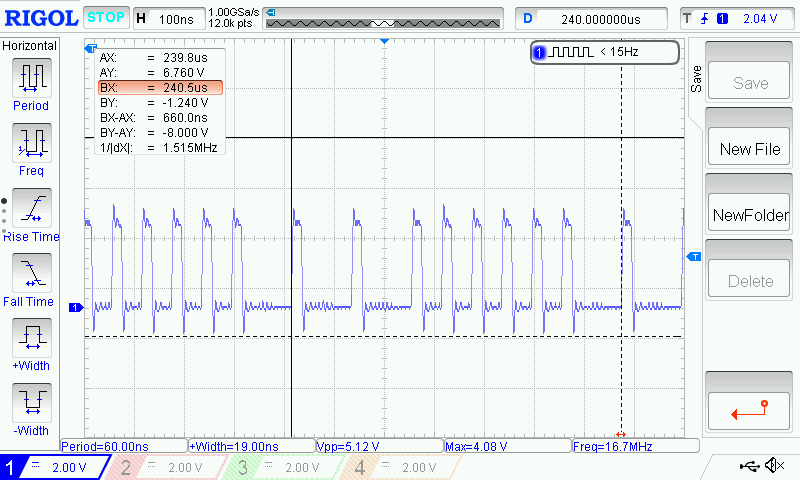
\includegraphics[scale=0.5]{instr_clk_impl} }}%
    \qquad
    \subfloat[Xilinx iSim simulation view of the \textit{q\_debug\_instr\_clk} signal.]{{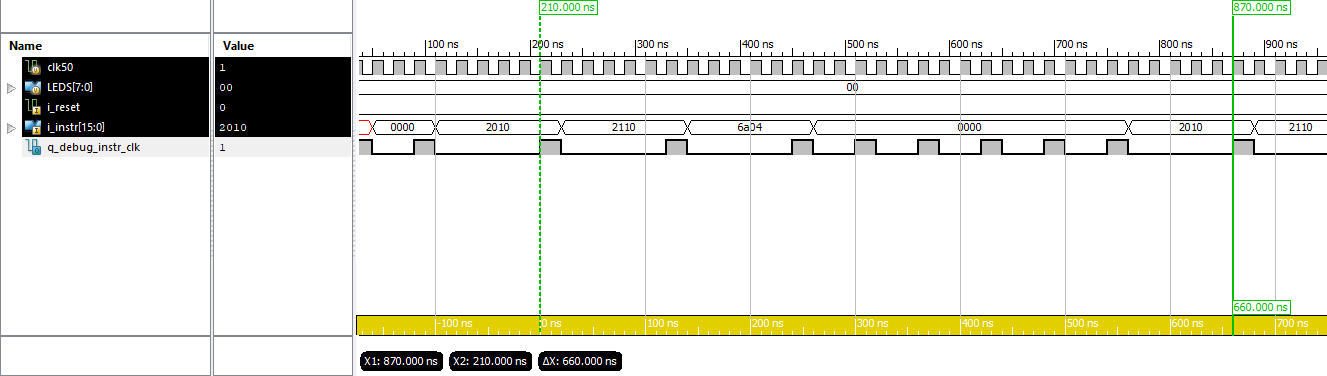
\includegraphics[scale=0.5]{instr_clk_sim} }}%
    \caption{Initial real-hardware implementation on the MiniSpartan6+ (XC6SLX9-3FTG256) development board showing timing of the \textit{q\_debug\_instr\_clk} signal. This signal is a 1 clock pulse indicating the start of an instruction cycle. In this example, instructions: MOVI \$10, \%Ra; MOVI \$10, \%Rb; and CMP \%Rc, \%Ra, \%Rb followed by 6 NOP instructions, are used.\newline\newline
    We can see that both implementations have a matching 660ns delay between instruction cycles for the same instructions, indicating that the real-hardware FPGA implementation is working correctly.}
    \label{fig:h5_impl}
\end{figure}

\newpage
\subsection*{Highlight 7}\label{inc:compiler_output}
Compiler input file contents:
\begin{minted}
[
frame=lines,
linenos
]
{python}
def foo() {
    10 + 1;
}

def main() {
    32;
    foo();
}
\end{minted}

Compiler output machine code (pre-optimisation, post assembling):
\begin{minted}
[
frame=lines,
linenos
]
{text}
0x00    ADDI    $-1,    Sp      4fff    Function/sf entry
0x01    SW      Bp,     +0(Sp)  16e0    (null)
0x02    MOV     Bp,     Sp      1ee0    main
0x03    MOVI    $20,    Ax      2020    NUMBER
0x04    MOVI    $9,     Cx      2209    Create return address
0x05    ADDI    $-1,    Sp      4fff    (null)
0x06    SW      Cx,     +0(Sp)  12e0    PUSH
0x07    MOVI    $d,     Cx      220d    call
0x08    JMP     Cx              6200    JMP
0x09    MOV     Sp,     Bp      1fc0    Function/sf exit
0x0A    LW      Bp,     +0(Sp)  0ee0    POP
0x0B    ADDI    $+1,    Sp      4f01    (null)
0x0C    HALT                    9000    MAIN HALT
------------------------------------
0x0D    ADDI    $-1,    Sp      4fff    Function/sf entry
0x0E    SW      Bp,     +0(Sp)  16e0    (null)
0x0F    MOV     Bp,     Sp      1ee0    foo
0x10    MOVI    $a,     Ax      200a    NUMBER
0x11    ADDI    $-1,    Sp      4fff    (null)
0x12    SW      Ax,     +0(Sp)  10e0    PUSH
0x13    MOVI    $1,     Ax      2001    NUMBER
0x14    LW      Cx,     +0(Sp)  0ae0    POP
0x15    ADDI    $+1,    Sp      4f01    (null)
0x16    ADD     Ax,     Cx      4040    BIN ADD
0x17    MOV     Sp,     Bp      1fc0    Function/sf exit
0x18    LW      Bp,     +0(Sp)  0ee0    POP
0x19    ADDI    $+1,    Sp      4f01    (null)
0x1A    LW      Cx,     +0(Sp)  0ae0    POP
0x1B    ADDI    $+1,    Sp      4f01    (null)
0x1C    JMP     Cx              6200    FUNC RETURN to CALL
\end{minted}

\newpage
\section{Risks and Challenges}
{\color{red} Urgent risks}\newline
{\color{orange} New risks}\newline
{\color{purple} Existing risks}\newline
{\color{gray} Resolved risks}

\subsection{Project Management}
\begin{itemize}
\item{{\color{gray} RC4: Schedule overrun. A gantt time chart has been created to better visualize task durations, requirements, and dependencies.}}
\end{itemize}

\subsection{CPU Core}
\begin{itemize}
\item{{\color{purple} RC5: Complex memory operations (PUSH, POP) may require multiple instructions. PUSH/POP might be split into: (1) Inc/dec stack pointer; (2) Read RAM[stack pointer]. The compiler will be able to resolve this issue.}}
\item{
{\color{orange} RC6: UART FIFO fills up too quickly, resulting in bad output.}
}
\end{itemize}


\subsection{Compiler}
There are currently no risks/challenges for the compiler.

\subsection{Other}
There are currently no additional risks/challenges.


\newpage
\bibliography{prco304_h4} 
\end{document}